\section{Numerical Validation}

The passive baseline was checked against geometry identities, synaptic normalization, current signs, matrix limits, timestep refinement, high-synapse stability, and Backward Euler versus Crank-Nicolson agreement. The baseline validation script generated the passive source data and classified all representative reference target values as passing predefined target-case tolerances. The most stringent target-case tolerance class means absolute error $\leq0.005$ or relative error $\leq2\%$, not bitwise equality.

Phase 4 added an independent direct-matrix benchmark for the passive three-compartment baseline reference cases. The benchmark independently parsed the baseline parameters, recomputed capacitance/leak/neck terms and the double-exponential synaptic conductance, assembled the passive matrices, and solved the Backward Euler system without calling the production passive simulation function as its benchmark engine. Compared with existing SPINE trace CSVs, the maximum all-trace absolute difference was $1.25\times10^{-13}$ mV, the maximum head-amplitude difference was $1.42\times10^{-14}$ mV, and the maximum $\Ghd$ difference was $7.55\times10^{-15}$.

Phase 4 also checked DC analytic limits. The spine-omitted two-node load formula gave $\Rin=144.48669201520912$ M$\Omega$, and the direct DC solve gave 144.48669201520914 M$\Omega$. Divider predictions for the low, intermediate, and high reference cases were 0.9912648, 0.8970688, and 0.4306959. The zero-neck and very-large-neck limiting cases approached local transfer values of 1 and 0, respectively.

The BE-versus-CN reference-case comparison remains an internal scheme-consistency check. Across the three baseline reference cases, the maximum peak differences were 0.00203 mV for $\Ah$, 0.000534 mV for $A_d$, 0.000189 mV for $A_s$, 0.000500 for $\Ghd$, and 0.000180 for $\Ghs$. The maximum trace voltage difference was 0.112 mV in the high-SMI case.

Passive morphology validation included sparse versus dense equivalence, spatial convergence, sinusoidal impedance validation, logarithmic-chirp impedance validation, and distributed-neck comparisons. Sinusoidal validation produced maximum relative amplitude error 0.0054. Chirp validation produced maximum relative amplitude error 0.072. Spatial convergence passed at the 16-versus-32 segment comparison with relative $\Ghs$ difference 0.014.

Active validation included AMPA peak normalization, NMDA magnesium-block monotonicity, NMDA current-voltage relief, active-current sign checks, gate bounds, positive gate time constants, resting-state stability, timestep refinement, limiting-case solver comparison, strong-drive stability, and active unit checks. All 12 active validation rows passed.

NEURON was unavailable in the Phase 4 execution environment. No NEURON result is claimed, and NEURON is not a runtime dependency of SPINE.

\begin{figure}[!htbp]
\centering
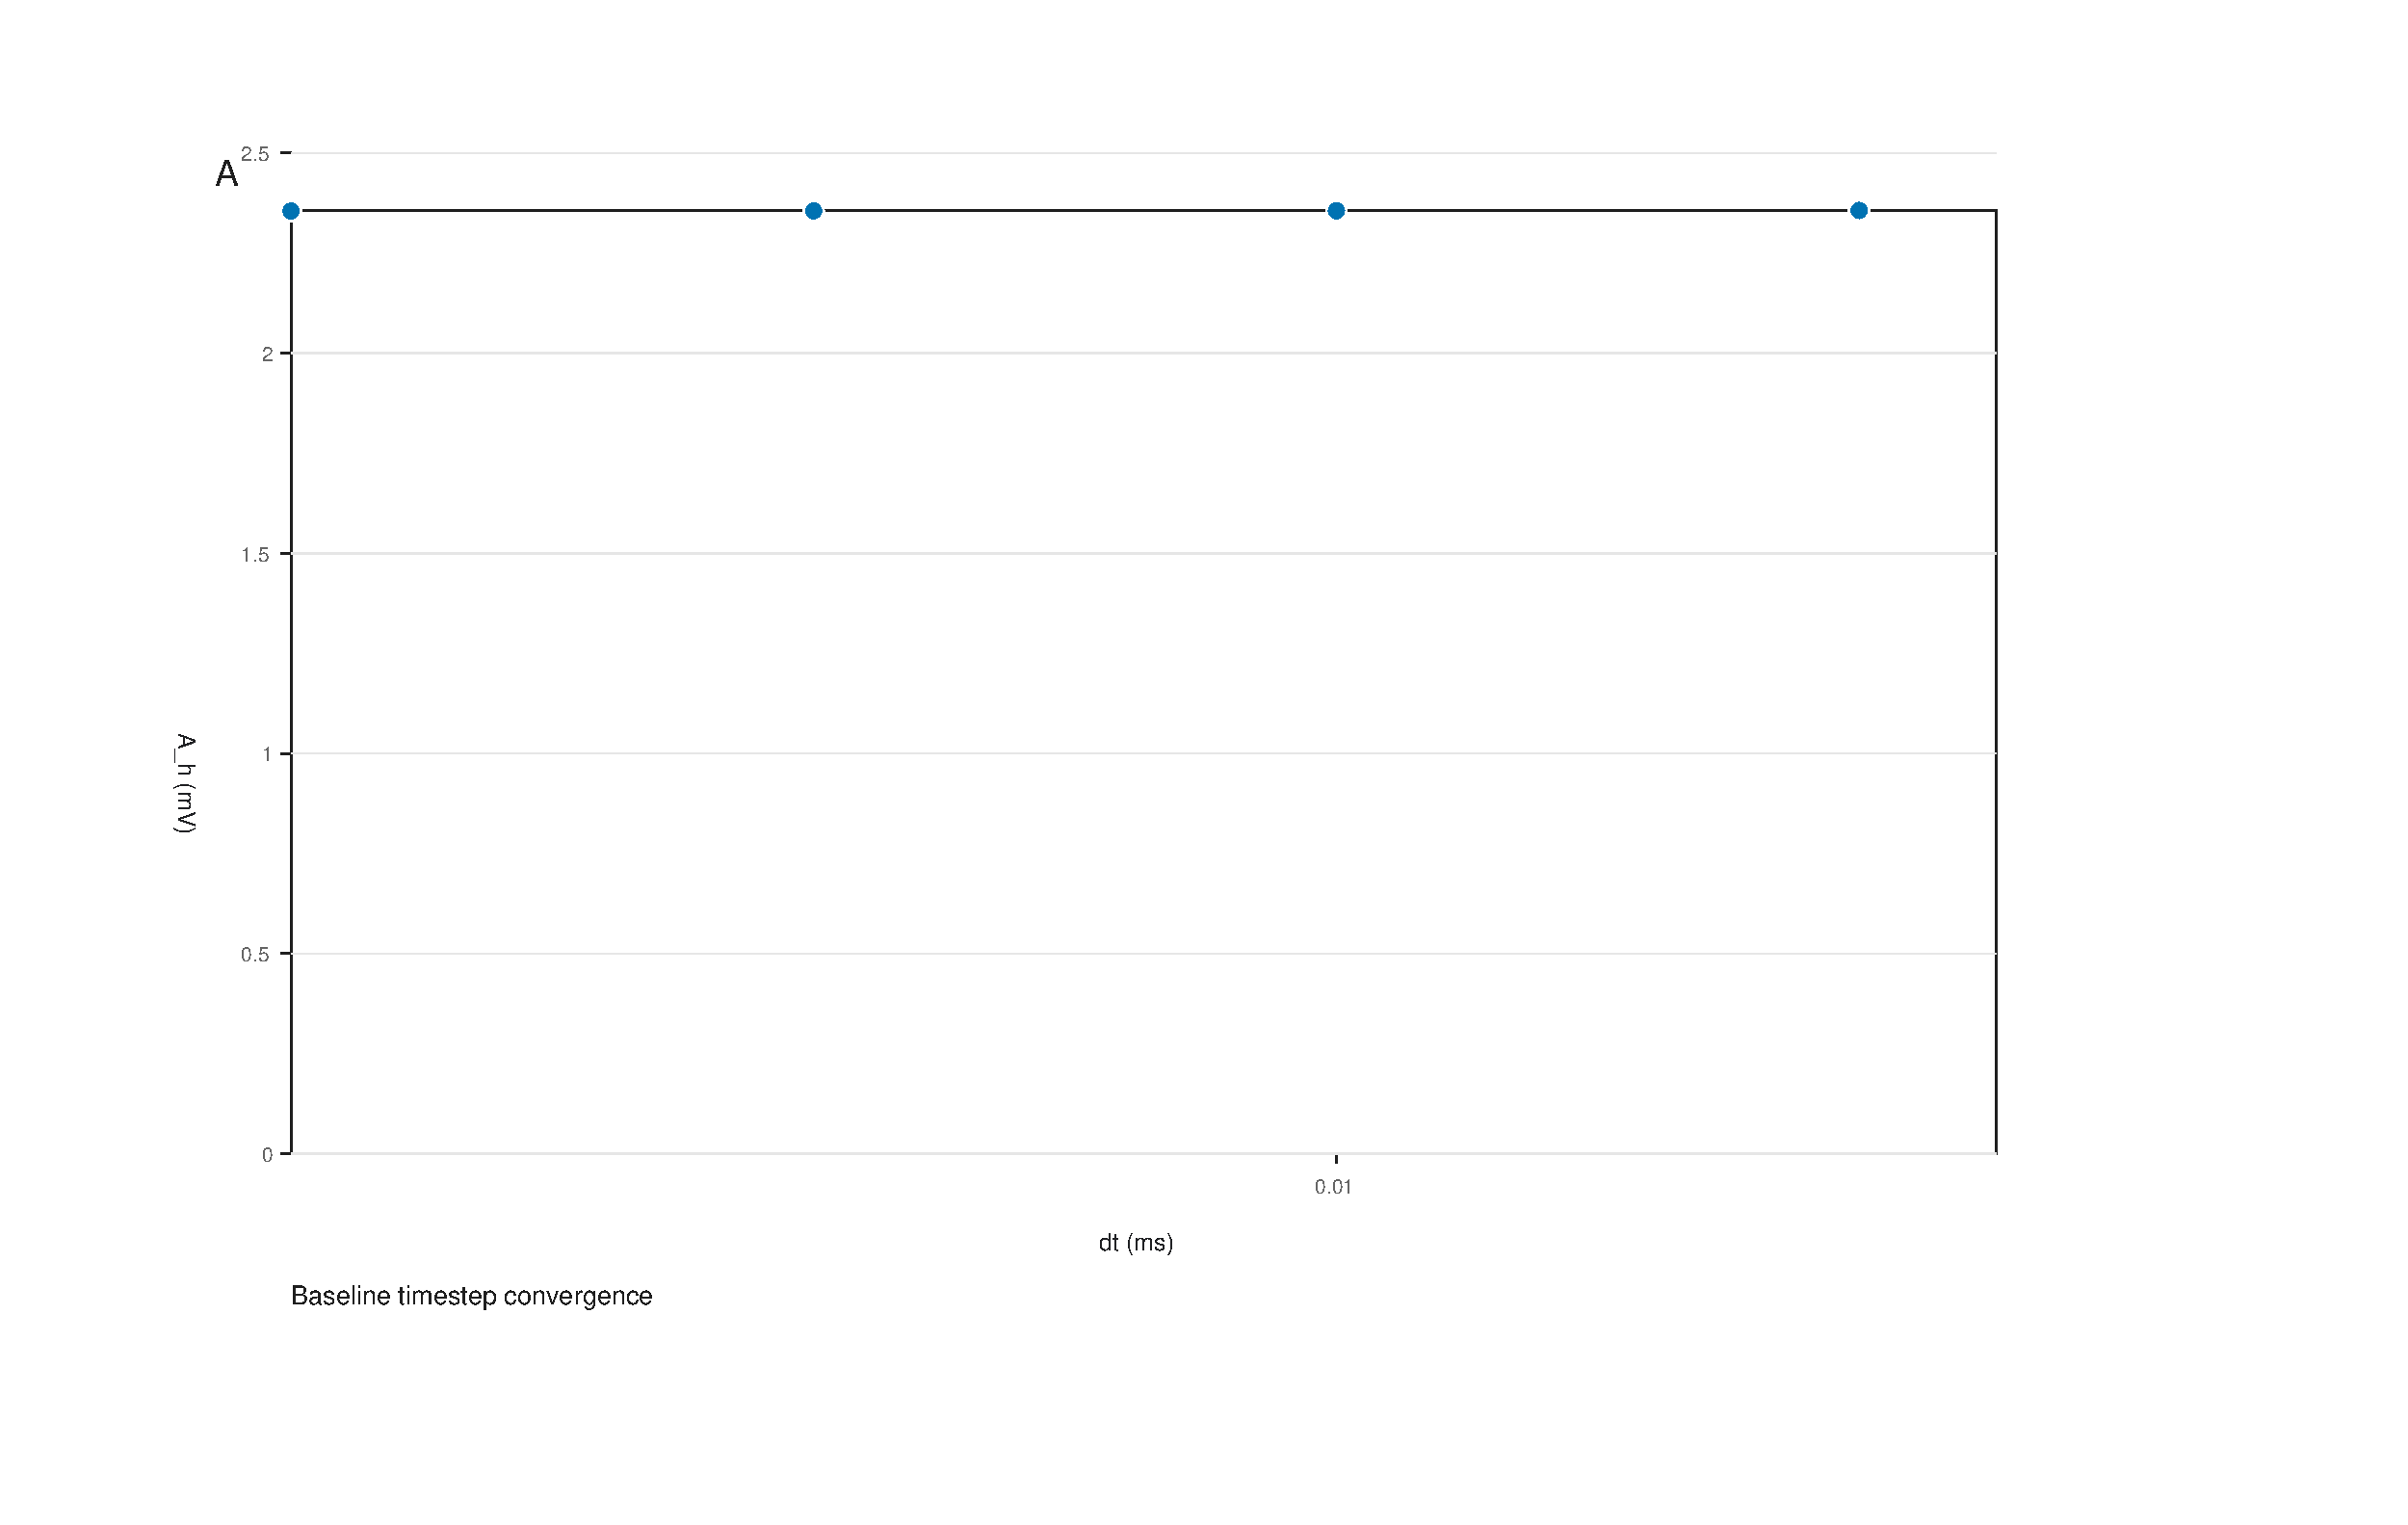
\includegraphics[width=0.85\textwidth,keepaspectratio]{../figures_publication/FigS2_dt_convergence.pdf}
\caption{\textbf{Figure S2.} Timestep convergence for the baseline-reference intermediate condition. The panel reports the audited head-amplitude convergence check used for numerical validation.}
\label{fig:s2_dt}
\end{figure}

\begin{figure}[!htbp]
\centering
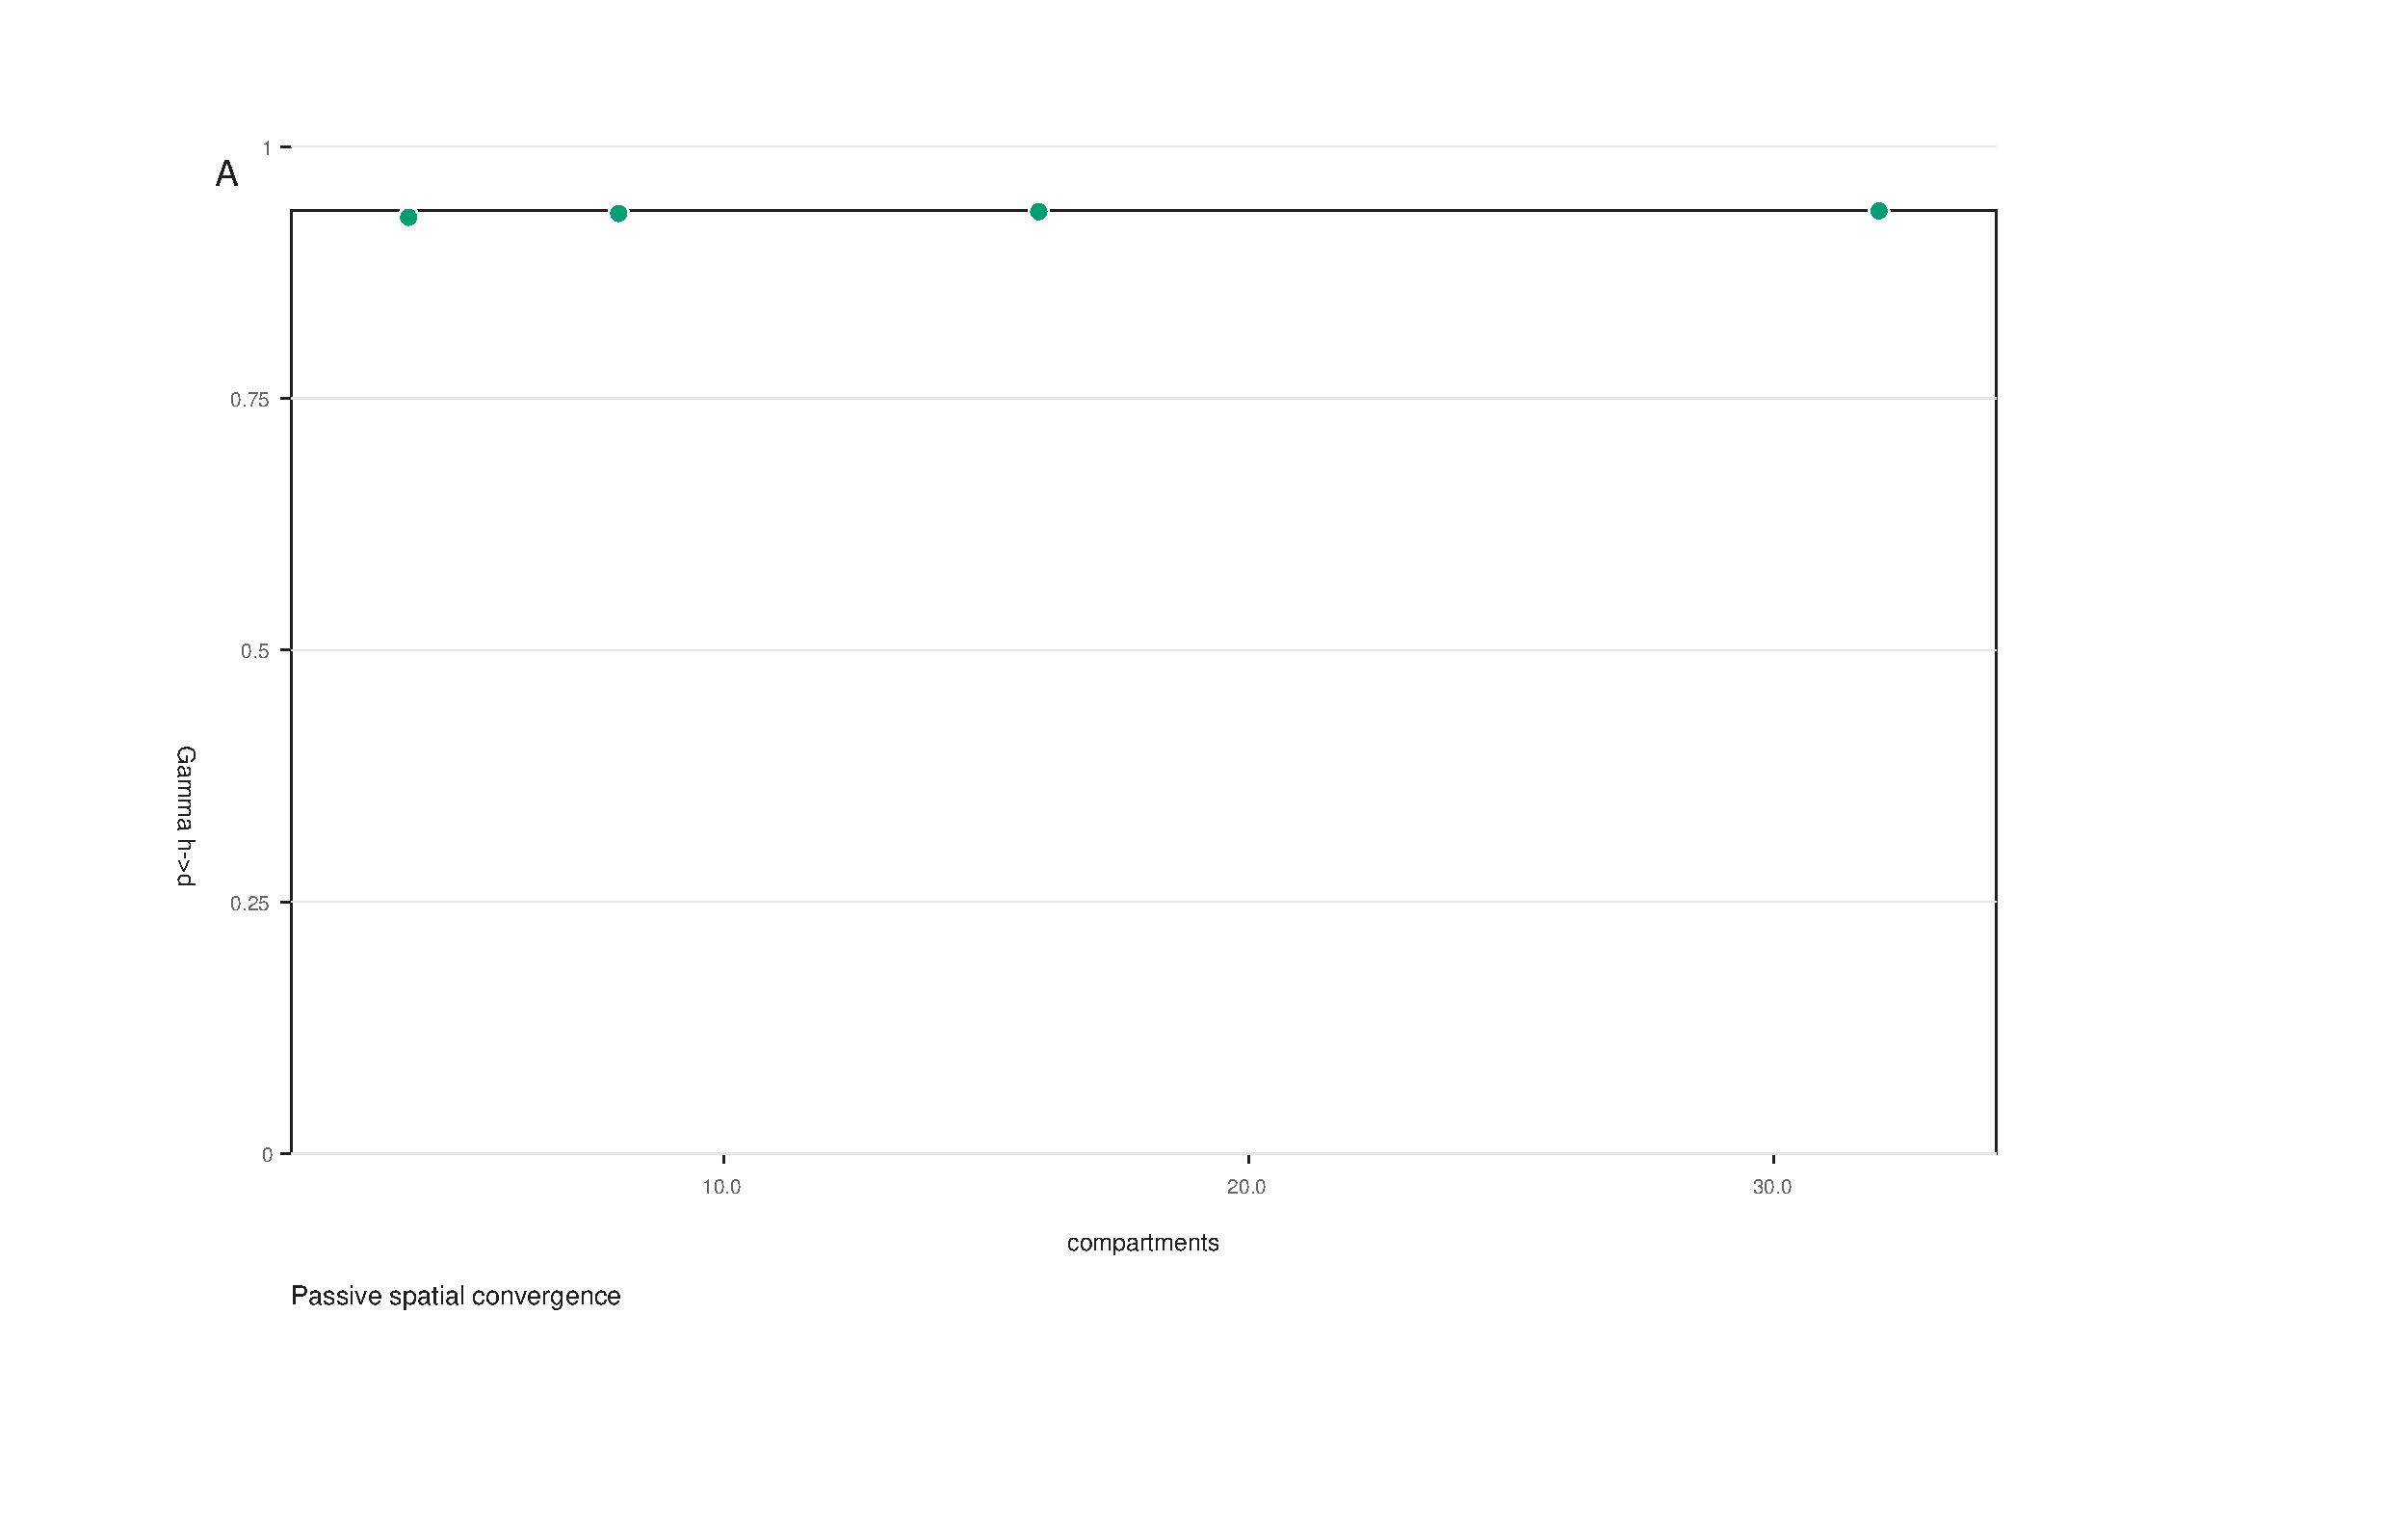
\includegraphics[width=0.85\textwidth,keepaspectratio]{../figures_publication/FigS3_spatial_convergence.pdf}
\caption{\textbf{Figure S3.} Spatial convergence for the passive morphology engine. The panel shows the dependence of local transfer on compartment discretization.}
\label{fig:s3_spatial}
\end{figure}

\begin{figure}[!htbp]
\centering
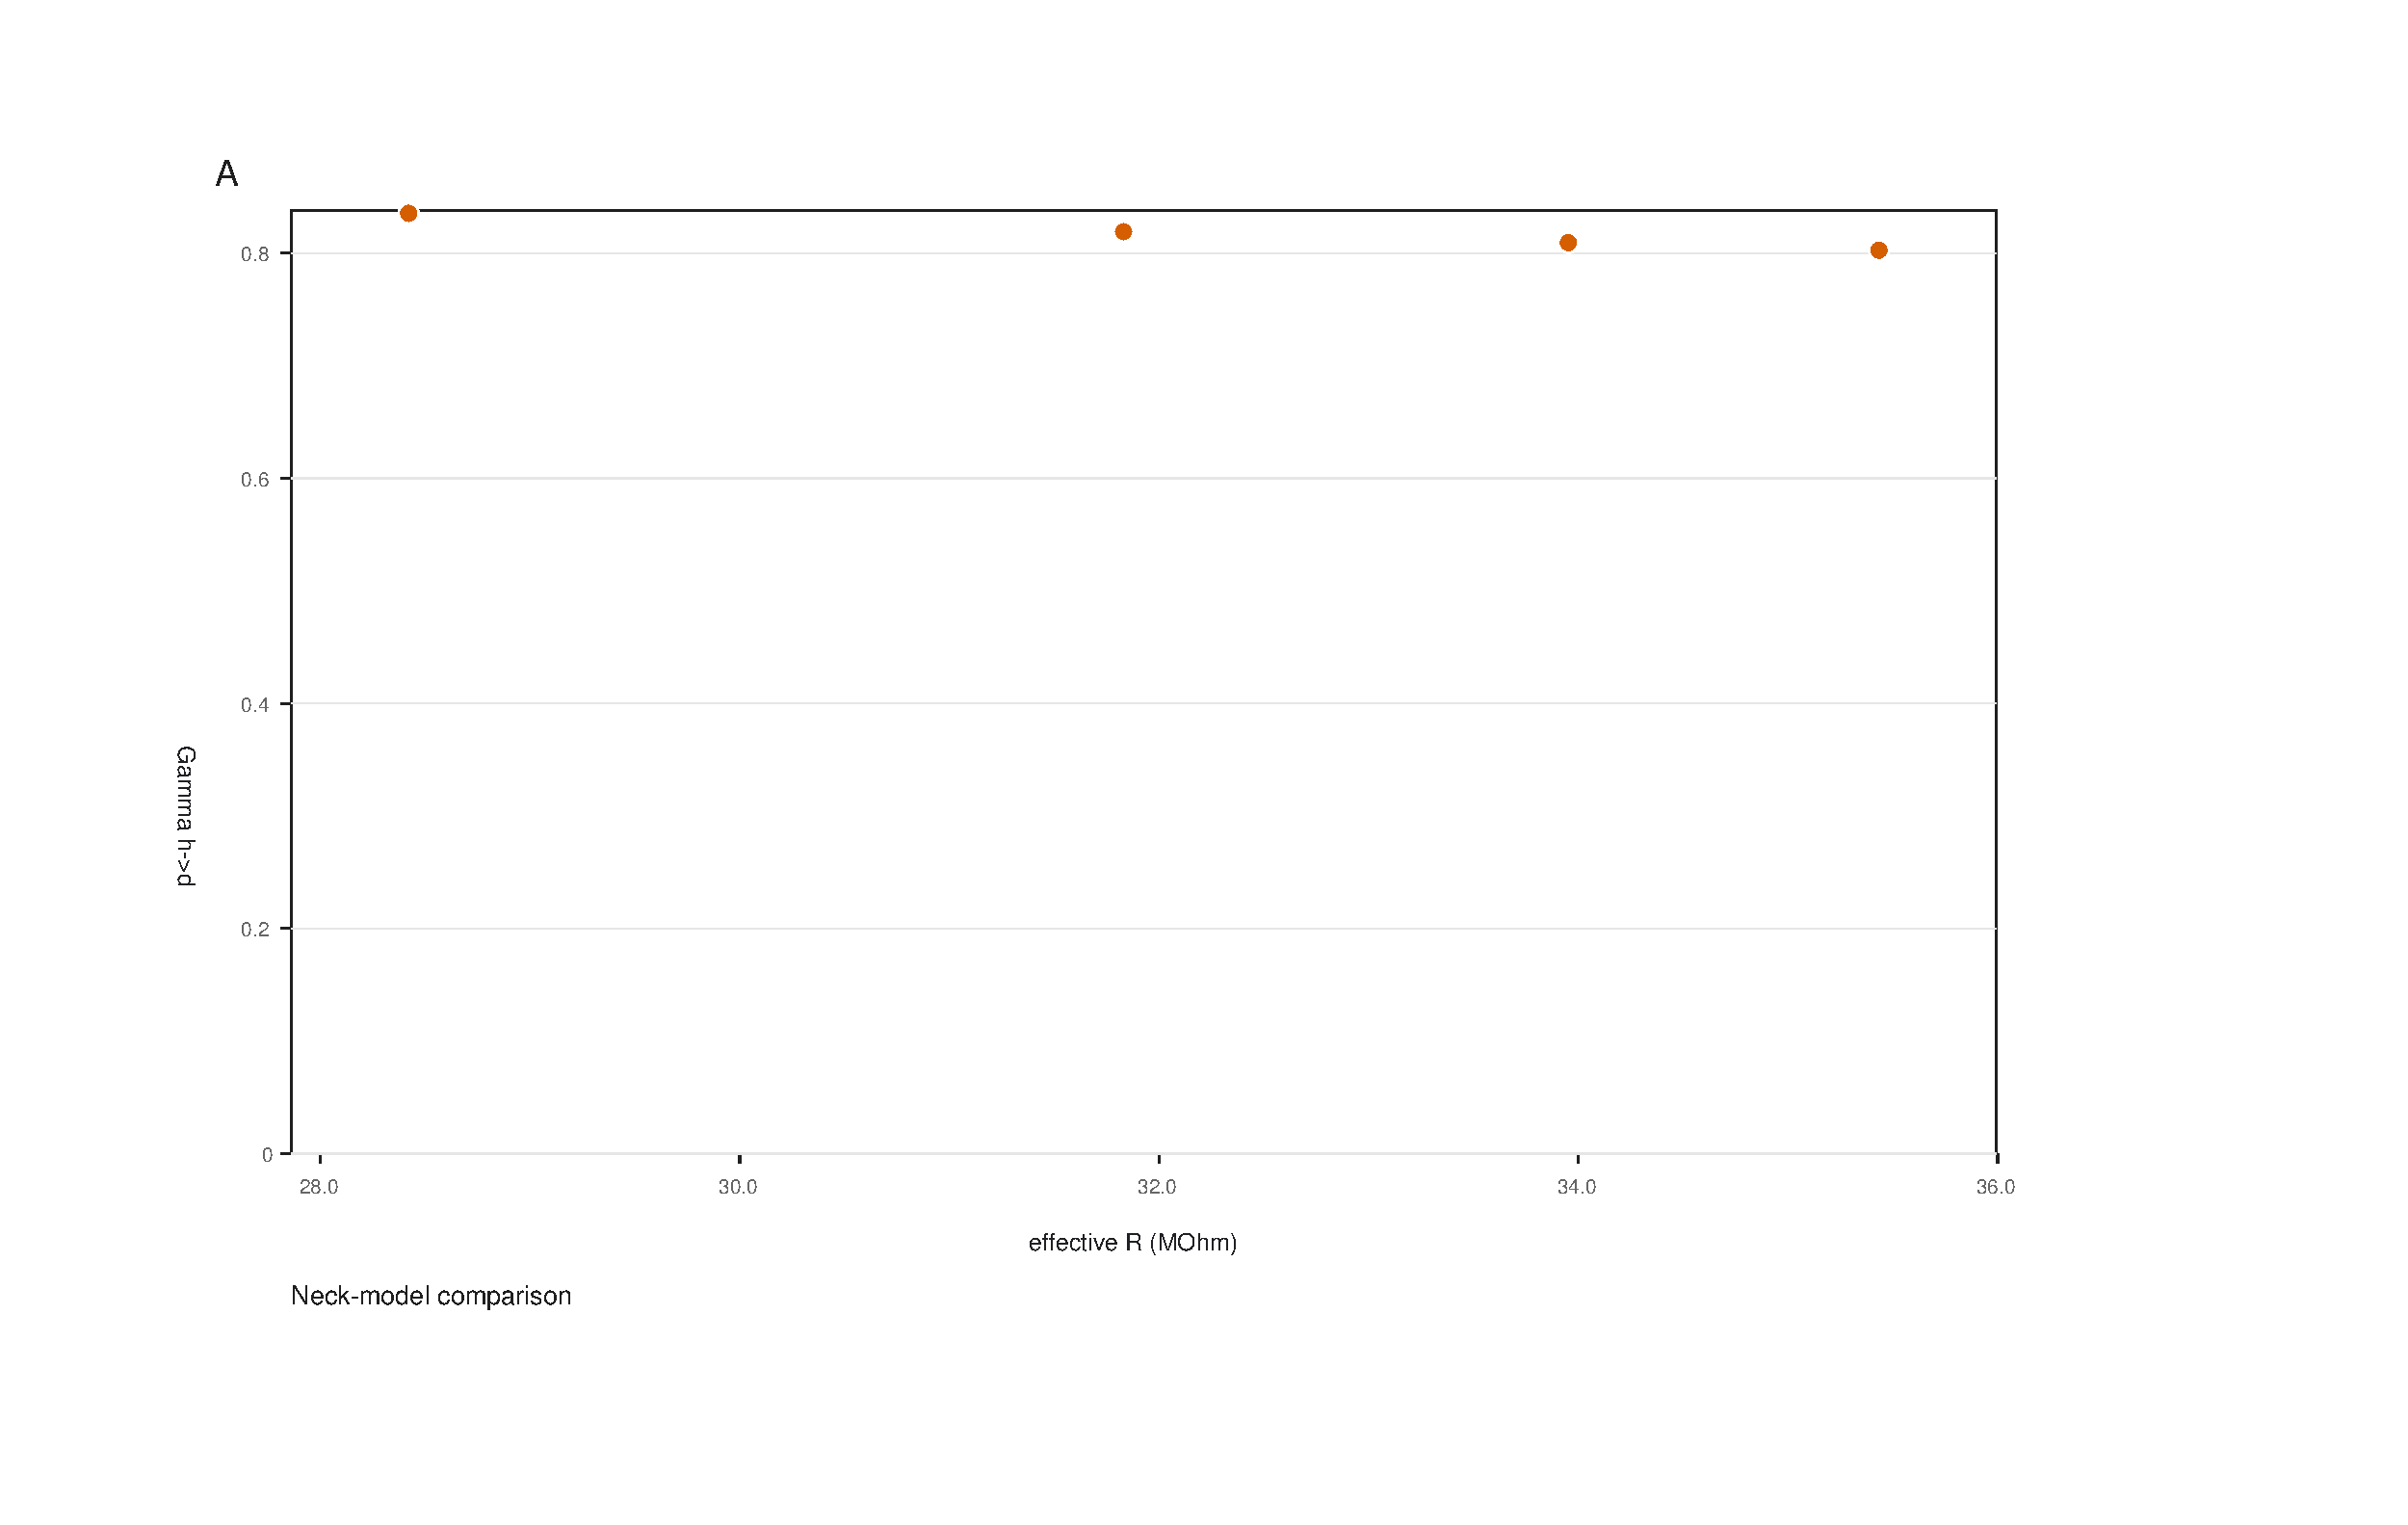
\includegraphics[width=0.85\textwidth,keepaspectratio]{../figures_publication/FigS4_neck_models.pdf}
\caption{\textbf{Figure S4.} Lumped and distributed neck-model comparisons. The panel contrasts effective neck resistance with local transfer for audited passive neck variants.}
\label{fig:s4_neck}
\end{figure}
